\documentclass[11pt,letterpaper,oneside]{report}
\usepackage[T1]{fontenc}
\usepackage[utf8]{inputenc}
\usepackage[english]{babel}
\usepackage{lmodern}
\usepackage{microtype}
\usepackage[margin=0.86in,headheight=16pt]{geometry}
\usepackage[table,dvipsnames]{xcolor}
\usepackage{graphicx}
\usepackage{booktabs,tabularx,longtable,array}
\usepackage{enumitem}
\usepackage{titlesec}
\usepackage{fancyhdr}
\usepackage{hyperref}
\usepackage{xurl}
\Urlmuskip=0mu plus 1mu\relax
\usepackage{tcolorbox}
\usepackage{listings}
\usepackage{tikz}
\usetikzlibrary{arrows.meta,positioning,shapes.geometric,fit,calc}
\usepackage{needspace}
\usepackage{amssymb}
\definecolor{ink}{HTML}{14253A}
\definecolor{navy}{HTML}{17385D}
\definecolor{blue}{HTML}{20739A}
\definecolor{pale}{HTML}{ECF4F8}
\definecolor{green}{HTML}{1D6C5C}
\definecolor{softgreen}{HTML}{EEF8F4}
\definecolor{border}{HTML}{D4DFE7}
\definecolor{grey}{HTML}{506174}
\hypersetup{colorlinks=true,linkcolor=navy,urlcolor=blue,pdfauthor={Micro-Frontend Engineering Documentation Suite}}
\titleformat{\chapter}[display]{\normalfont\sffamily\bfseries\color{ink}}{\Large\color{blue}\MakeUppercase{\chaptername} \thechapter}{8pt}{\Huge}
\titlespacing*{\chapter}{0pt}{-10pt}{24pt}
\titleformat{\section}{\Large\sffamily\bfseries\color{navy}}{\thesection}{0.7em}{}
\titleformat{\subsection}{\large\sffamily\bfseries\color{navy}}{\thesubsection}{0.6em}{}
\setlist[itemize]{itemsep=3pt,topsep=5pt,leftmargin=1.6em}
\setlist[enumerate]{itemsep=4pt,topsep=5pt,leftmargin=1.8em}
\pagestyle{fancy}\fancyhf{}
\fancyhead[L]{\footnotesize\sffamily MICRO-FRONTEND ENGINEERING SUITE}
\fancyhead[R]{\footnotesize\sffamily\docshort}
\fancyfoot[L]{\footnotesize\color{grey}Engineering edition | October 2026}
\fancyfoot[R]{\footnotesize\thepage}
\renewcommand{\headrulewidth}{0.35pt}
\renewcommand{\arraystretch}{1.2}
\setlength{\emergencystretch}{2em}
\lstdefinestyle{eng}{basicstyle=\ttfamily\footnotesize,keywordstyle=\color{navy}\bfseries,commentstyle=\color{grey},stringstyle=\color{green},breaklines=true,breakatwhitespace=false,columns=fullflexible,keepspaces=true,showstringspaces=false,frame=single,rulecolor=\color{border},backgroundcolor=\color{pale},xleftmargin=5pt,xrightmargin=5pt,aboveskip=10pt,belowskip=10pt,captionpos=b}
\lstdefinelanguage{JavaScript}{morekeywords={const,let,var,require,return,async,await,import,export,default,function,try,catch,new,true,false,undefined,module},sensitive=true,morecomment=[l]//,morestring=[b]',morestring=[b]"}
\lstset{style=eng}
\newtcolorbox{sourcebox}{colback=pale,colframe=border,arc=2pt,boxrule=0.6pt,left=8pt,right=8pt,top=7pt,bottom=7pt}
\newtcolorbox{engineerbox}{colback=softgreen,colframe=green!45,arc=2pt,boxrule=0.6pt,left=8pt,right=8pt,top=7pt,bottom=7pt}
\newcommand{\based}[1]{\begin{sourcebox}\textbf{BOOK-GROUNDED CONCEPT}\\#1\end{sourcebox}}
\newcommand{\added}[1]{\begin{engineerbox}\textbf{ENGINEERING EXTENSION}\\#1\end{engineerbox}}
\newcommand{\term}[1]{\textbf{\color{navy}#1}}
\newcommand{\criterion}[1]{\textbf{Acceptance:} #1}
\newcommand{\book}{\emph{Building Micro-Frontends}, 2nd ed.}
\newcommand{\refs}{\chapter*{References and Provenance}\addcontentsline{toc}{chapter}{References and Provenance}
\begin{enumerate}[leftmargin=*]
\item \textbf{Primary source:} Luca Mezzalira, \emph{Building Micro-Frontends: Distributed Systems for the Frontend}, 2nd ed., O'Reilly Media, published November 2025 (copyright 2026), ISBN 978-1-098-17078-3. Chapter and printed-page references are included throughout. This suite paraphrases and synthesizes concepts; it does not reproduce the book.
\item \textbf{Engineering extension:} Webpack Module Federation reference: \url{https://webpack.js.org/plugins/module-federation-plugin}.
\item \textbf{Engineering extension:} Next.js multi-zones: \url{https://nextjs.org/docs/app/guides/multi-zones}. Details are version-sensitive and must be checked against the deployed framework version.
\item \textbf{Engineering extension:} OWASP Application Security Verification Standard 5.0: \url{https://owasp.org/www-project-application-security-verification-standard/}.
\item \textbf{Engineering extension:} GitHub Actions secure use reference: \url{https://docs.github.com/en/actions/reference/security/secure-use}.
\end{enumerate}}

\titleclass{\chapter}{straight}\titleformat{\chapter}[hang]{\huge\sffamily\bfseries\color{navy}}{\thechapter}{.7em}{}\titlespacing*{\chapter}{0pt}{24pt}{13pt}
\newcommand{\docshort}{TECHNICAL REFERENCE}
\begin{document}
\begin{titlepage}\thispagestyle{empty}
\vspace*{1.1in}{\Huge\sffamily\bfseries\color{navy} Micro-Frontend Technical Reference\par}
\vspace{18pt}{\Large\sffamily\color{blue} Architecture concepts, runtime models, system qualities, and operational standards\par}
\vspace{27pt}\noindent\color{blue}\rule{0.75\textwidth}{1.4pt}
\vspace{23pt}\par{\large\sffamily A companion to Luca Mezzalira's \emph{Building Micro-Frontends}, Second Edition}\par
\vfill\noindent\textbf{Document series:} Micro-Frontend Software Architecture and Engineering\\
\textbf{Version:} 1.0 \quad \textbf{Prepared:} October 2026\\
\textbf{Production format:} pdfLaTeX-compatible standalone source\\
\textbf{Scope:} Original synthesis plus explicitly identified engineering extensions
\end{titlepage}
\pagenumbering{roman}\tableofcontents\clearpage\pagenumbering{arabic}

\chapter{Scope, Vocabulary, and Architecture Principles}
\based{Chapters 1--3, pp. 1--113, introduce distributed frontends as independently deliverable business-domain slices, not merely UI components. The book emphasizes domain boundaries, autonomous teams, composition, routing, communication, automation, and observability.}
\section{Definition and applicability}
A \term{micro-frontend} is an independently developed, tested, and deployable frontend capability aligned with a business subdomain and owned by an accountable team. A \term{component} is a UI building block; component reuse does not by itself create independent business ownership or delivery. A \term{frontend monolith} can be entirely suitable when few teams, uncomplicated delivery, and limited domain coupling make a distributed architecture more expensive than beneficial.
\section{Design principles}
\begin{longtable}{p{.27\linewidth}p{.65\linewidth}}\toprule Principle & Architectural interpretation \\\midrule
Business-domain modeling & Prefer boundaries based on stable user capabilities and bounded contexts over framework or UI-widget boundaries.\\
Automation culture & Every domain supplies reproducible builds, repeatable testing, and unattended promotion.\\
Encapsulation & Publish an explicit public contract; conceal private source, state structures, and persistence details.\\
Decentralization & Delegate local technical decisions to stream-aligned teams while sharing minimal platform invariants.\\
Independent deployment & Promote one domain without synchronizing unrelated domains, subject to compatibility tests.\\
Failure isolation & A failing remote should degrade only its owned capability where the composition model permits.\\
Observability & Trace the complete user journey across shell, remotes, edge, and API boundaries.\\\bottomrule\end{longtable}
\added{A practical adoption test is whether independent delivery and clear domain ownership offset added runtime integration, dependency governance, browser performance, and production operations. This is an engineering decision rule, not a guarantee that decomposition improves throughput.}
\chapter{The Four Architecture Decisions}
\based{Chapter 2, pp. 17--37, names four decision areas: define a micro-frontend, compose micro-frontends, route between micro-frontends, and communicate between them. The four decisions should be written down before choosing a federation library.}
\section{Boundary definition}
A \term{vertical split} gives a micro-frontend a complete user capability or route range and normally loads one at a time. A \term{horizontal split} places independently owned capabilities together on a single page. Mixed models are possible; document ownership boundaries per view.
\section{Composition}
\begin{tabularx}{\linewidth}{p{.19\linewidth}X X}\toprule Model & Strength & Principal costs \\\midrule
Client-side & Independent browser loading; interactive composition & JS startup, dependency collision, remote availability, hydration mismatches\\
Server-side & HTML available early; origin controls composition & Server coordination, cache invalidation, streaming errors, infrastructure overhead\\
Edge-side & Proximity to users; CDN distribution & Edge portability, cache coherence, personalization risks\\
Route-based & Simple ownership boundaries and fault containment & Full navigation across zones; shared shell consistency\\\bottomrule\end{tabularx}
\section{Routing and communication}
Use a centralized route registry for ownership, navigation, auth entry, and fallback behavior, but do not create a giant business-logic shell. Prefer \term{URL and navigation} for coarse-grained workflow transitions, \term{typed custom events} for narrow cross-domain signals, and \term{API-owned server state} for durable truth. Avoid unconstrained shared mutable frontend stores.
\chapter{Reference Architecture}
\begin{center}
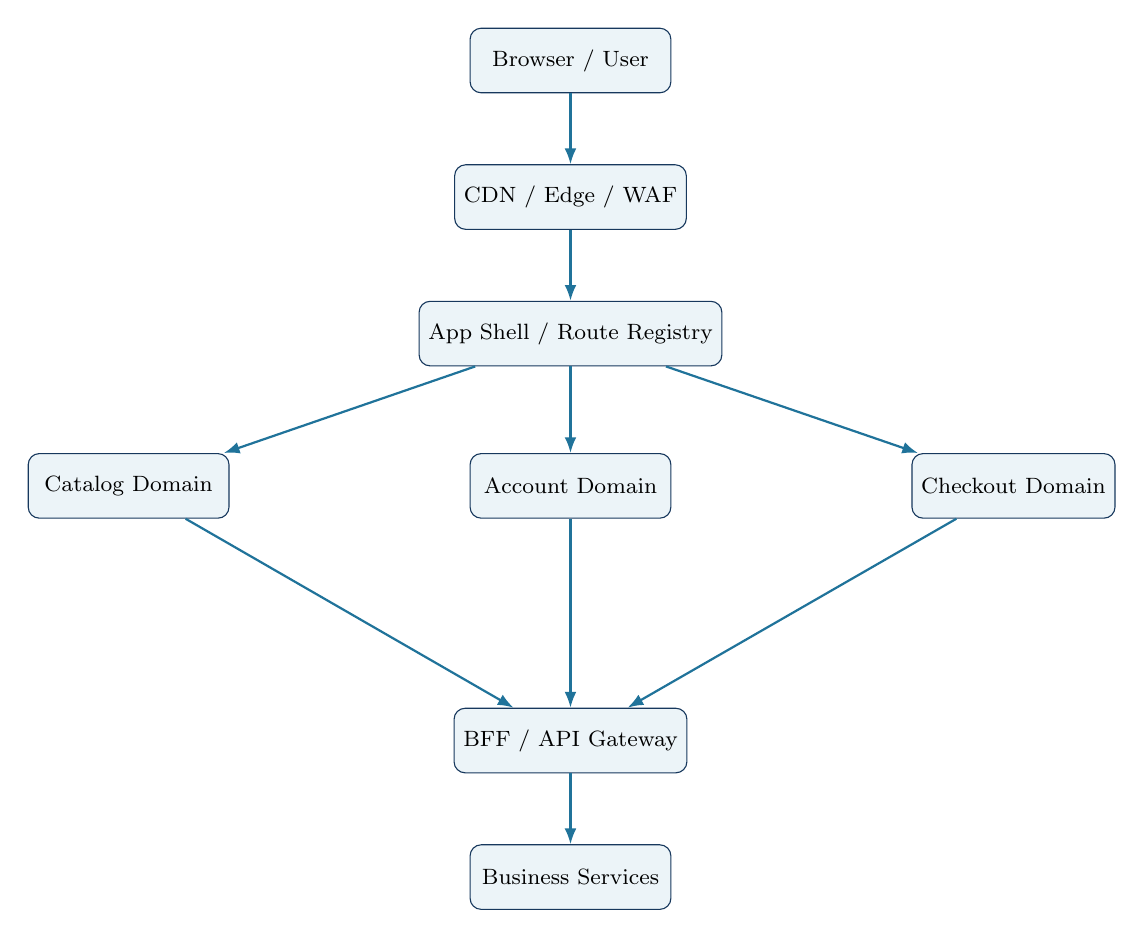
\begin{tikzpicture}[node distance=9mm and 12mm, every node/.style={font=\footnotesize}, box/.style={draw=navy,rounded corners,fill=pale,align=center,minimum width=2.55cm,minimum height=.82cm}, arr/.style={-{Latex[length=2mm]},thick,draw=blue}]
\node[box] (user) {Browser / User};
\node[box,below=of user] (edge) {CDN / Edge / WAF};
\node[box,below=of edge] (shell) {App Shell / Route Registry};
\node[box,below left=11mm and 24mm of shell] (a) {Catalog Domain};
\node[box,below=11mm of shell] (b) {Account Domain};
\node[box,below right=11mm and 24mm of shell] (c) {Checkout Domain};
\node[box,below=24mm of b] (api) {BFF / API Gateway};
\node[box,below=of api] (svc) {Business Services};
\draw[arr] (user)--(edge);\draw[arr](edge)--(shell);
\foreach \x in {a,b,c}{\draw[arr] (shell)--(\x);\draw[arr](\x)--(api);}
\draw[arr](api)--(svc);
\end{tikzpicture}
\end{center}
\noindent The diagram illustrates one valid implementation, not a universal requirement. The edge layer may route whole zones without browser federation; domain APIs may be separate instead of a shared gateway.
\section{Application shell ownership}
The shell owns initial bootstrap, stable navigation, runtime discovery, identity integration, global accessibility landmarks, telemetry wiring, top-level error handling, and degradation. It should not own domain checkout rules, account-edit state, or feature-specific transformation logic.
\section{Contracts between domains}
Define contracts for route prefixes, exported lifecycle (mount/unmount) or module signatures, auth context, events, design tokens, telemetry context, supported dependency ranges, and fallback UI. Every contract has an owner, version, consumer tests, and a deprecation policy.
\chapter{Composition and Runtime Techniques}
\section{Client-side Module Federation}
\based{Chapter 4, pp. 115--149, demonstrates client-side micro-frontends using Module Federation, an application shell, individual domain apps, incremental evolution, and caching.}
The host resolves remote modules from deployment-specific URLs. An explicit shared-dependency policy may reduce duplicate code but couples runtime compatibility. Audit \texttt{shared} singleton declarations, remote entry origins, cache headers, and fallback behavior. A remote import must have a timeout/error boundary where possible; module federation itself does not provide security isolation.
\section{Server rendering and multi-zones}
\based{Chapter 5, pp. 151--179, covers HTML fragments, URL partitioning, Next.js multi-zones, API design, SSR scalability, and multi-layer caching.}
Route-partitioned server applications can operate as autonomous zones. A reverse proxy sends each path to its owner; shared user identity must be validated server-side. Cross-zone navigations may be hard navigations. Fragment composition requires careful decisions about caching, document metadata, CSS, streaming, and failure handling.
\section{Web components, iframes, and fragments}
Web components establish browser-native custom elements and encapsulation tools, but do not independently define bounded contexts or solve business coupling. Iframes offer comparatively strong document isolation at the cost of navigation, resizing, focus management, analytics, and authentication friction. HTML fragment and edge composition require explicit trust boundaries before inserting remote markup.
\chapter{Backend Integration and Data Ownership}
\based{Chapter 9, pp. 237--268, presents service dictionaries, API gateways, backend-for-frontend (BFF), GraphQL federation, and API consistency.}
\section{Selection matrix}
\begin{tabularx}{\linewidth}{p{.25\linewidth}X X}\toprule Pattern & Best fit & Primary risk \\\midrule
BFF per experience & Client-specific orchestration / tailored response & Duplicate orchestration and unclear domain ownership\\
Domain API gateway & Policy, authentication entry, traffic control & Gateway becomes tightly coupled shared code\\
Service dictionary & Resolve APIs via an owned, versioned registry & Stale entries and misrouted consumers\\
GraphQL composition & Flexible typed read graph across domains & Resolver authorization, query costs, ownership ambiguity\\\bottomrule\end{tabularx}
\section{Nonnegotiable invariants}
Clients are untrusted. Authorization executes at trusted services, not merely in shell route guards. APIs validate input, issue correlated error codes, enforce quotas, and document ownership. Treat browser communication as a convenience mechanism, not a source of record. Avoid cross-domain synchronous request chains for a single first paint.
\chapter{Cross-Cutting Quality Attributes}
\begin{longtable}{p{.25\linewidth}p{.67\linewidth}}\toprule Attribute & Engineering verification \\\midrule
Performance & Per-route budgets for JS transferred, hydration/interaction, LCP/INP/CLS; test realistic devices and networks.\\
Availability & Test remote outage, stale cache, rollback, origin timeout, and degraded state.\\
Security & Verify authentication and server authorization, CSP, trusted remote origins, supply chain controls, XSS protections, and secure cookie settings.\\
Accessibility & Keyboard/focus transitions, landmarks, heading hierarchy, error recovery, contrast, and screen-reader flows across zone boundaries.\\
Operability & Correlation IDs, app/domain/release identifiers, error rate and latency signals, and release annotations in dashboards.\\
Maintainability & Domain ownership, coupling analysis, contract change reviews, dead dependency removal, and documented ADRs.\\\bottomrule\end{longtable}
\added{Use OWASP ASVS 5.0 for testable web-security requirements; performance targets and SLOs below should be selected by the organization, not presented as numbers mandated by the book.}
\chapter{Architecture Antipattern Catalog}
\based{Chapter 10, pp. 271--284, emphasizes confusion between micro-frontends and components, excessive shared state, governance-free proliferation, one-way dependency violations, and premature abstraction.}
\begin{longtable}{p{.25\linewidth}p{.29\linewidth}p{.35\linewidth}}\toprule Smell & Impact & Correction \\\midrule
UI widget as micro-frontend & Too many deployment units & Recompose around a business capability\\
Single global store & Hidden coupling across teams & Local state; durable state via domain APIs\\
Remote-to-remote internals & Coordinated releases & Contracts/events/anti-corruption layer\\
Unlimited framework freedom & Runtime and support burden & Platform guardrails plus justified exceptions\\
Shell as business monolith & Central release bottleneck & Keep shell a platform boundary\\
Over-sharing libraries & Version lockstep & Share small stable contracts/tokens only\\\bottomrule\end{longtable}
\chapter{Operational Definition of Done}
Each independently deployable domain has: (1) a named owner; (2) a business capability and route map; (3) documented contracts and compatibility; (4) a reproducible build and test evidence; (5) a risk-assessed security boundary; (6) automated deployment and rollback; (7) observability fields and dashboard; (8) accessibility and performance evidence; and (9) an ADR recording the most consequential trade-offs.

\refs
\end{document}
